\apendice{Manual de especificación de diseño}

\section{Diseño arquitectónico}
Este capítulo tiene como objetivo describir la estructura interna del sistema de entrenamiento desarrollado, así como el despliegue de la interfaz gráfica, mediante el uso de diagramas explicativos que representan el flujo de trabajo del modelo de segmentación.

En la Figura \ref{fig: diagrama_de_clases} se muestra el diagrama de clases que representa los principales componentes de la fase de entrenamiento.
\begin{figure}[h]
    \centering
    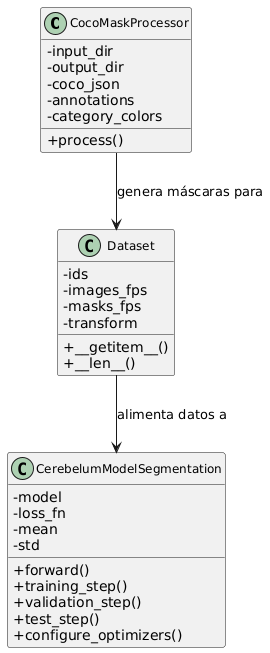
\includegraphics[width=0.5\textwidth]{img/diagrama1.png}
    \caption{Diagrama de clases del entrenamiento.}
    \label{fig: diagrama_de_clases}
\end{figure}

En la Figura \ref{fig: diagrama_interfaz} se muestra el diagrama de arquitectura funcional de la aplicación, que muestra el flujo de procesamiento desde la carga de la imagen hasta la descarga del informe en PDF, pasando por la segmentación automática y el cálculo de métricas.

\begin{figure}[h]
    \centering
    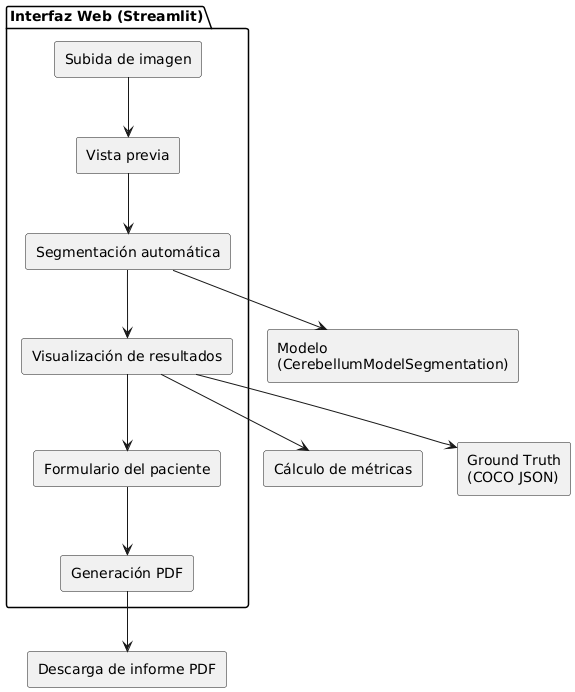
\includegraphics[width=
    \textwidth]{img/diagrama2.png}
    \caption{Arquitectura funcional de la interfaz Streamlit desarrollada.}
    \label{fig: diagrama_interfaz}
\end{figure}
